\documentclass{beamer}

\useoutertheme[subsection=false]{miniframes}
\usecolortheme{beaver}
\setbeamertemplate{navigation symbols}{}
\setbeamertemplate{footline}{}
\usepackage{graphicx}

\usepackage{url}
\usepackage{datetime}
\usepackage[export]{adjustbox}


\newcommand {\framedgraphic}[3] {
  \begin{frame}{#1}
    \vspace{-0.5cm}
    \begin{center}
      \includegraphics[width=0.9\textwidth,keepaspectratio]{#2}
    \end{center}
    \vspace{-1cm}
    \begin{center}
      #3
    \end{center}
  \end{frame}
}
\newcommand{\lectureDate}{\formatdate{27}{09}{2018}}

\setbeamertemplate{caption}{\raggedright\insertcaption\par}
\title{MATH211: Linear Methods I}
\author{Matthew Burke}
\date{\lectureDate}
\begin{document}

\frame{\titlepage}

\begin{frame}{Lecture on \lectureDate}
  \tableofcontents
\end{frame}

\section*{Last time}
\label{sec:Last-time}

\begin{frame}{Last time}
  \begin{itemize}
  \item Elementary matrices\vfill
  \item Elementary matrices as theoretical tool\vfill
  \item Matrix equations
  \end{itemize}
\end{frame}

\section{Determinants}

\begin{frame}
  \begin{beamercolorbox}[sep=12pt,center]{part title}
    \usebeamerfont{section title}\insertsection\par
  \end{beamercolorbox}
\end{frame}

\begin{frame}{Two dimensional determinants}
  The standard basis vectors get sent to the columns:\vfill
  \begin{equation*}
    \left[
      \begin{array}{cc}
        a&b\\
        c&d
      \end{array}
    \right]
    \left[
      \begin{array}{c}
        1\\
        0
      \end{array}
    \right] =
    \left[
      \begin{array}{c}
        a\\
        c
      \end{array}
    \right]\text{ and }
    \left[
      \begin{array}{cc}
        a&b\\
        c&d
      \end{array}
    \right]
    \left[
      \begin{array}{c}
        0\\
        1
      \end{array}
    \right] =
    \left[
      \begin{array}{c}
        b\\
        d
      \end{array}
    \right]
  \end{equation*}\vfill
  \begin{definition}
    The \emph{determinant
      \begin{equation*}
        det(A) = \left| A\right|
      \end{equation*}
      of any square matrix $A$} is the \emph{signed area} spanned by the columns of the matrix.
  \end{definition}
\end{frame}

\begin{frame}{Picture of two dimensional determinant}
  \begin{figure}
    \begin{columns}
      \column{.6\textwidth}
      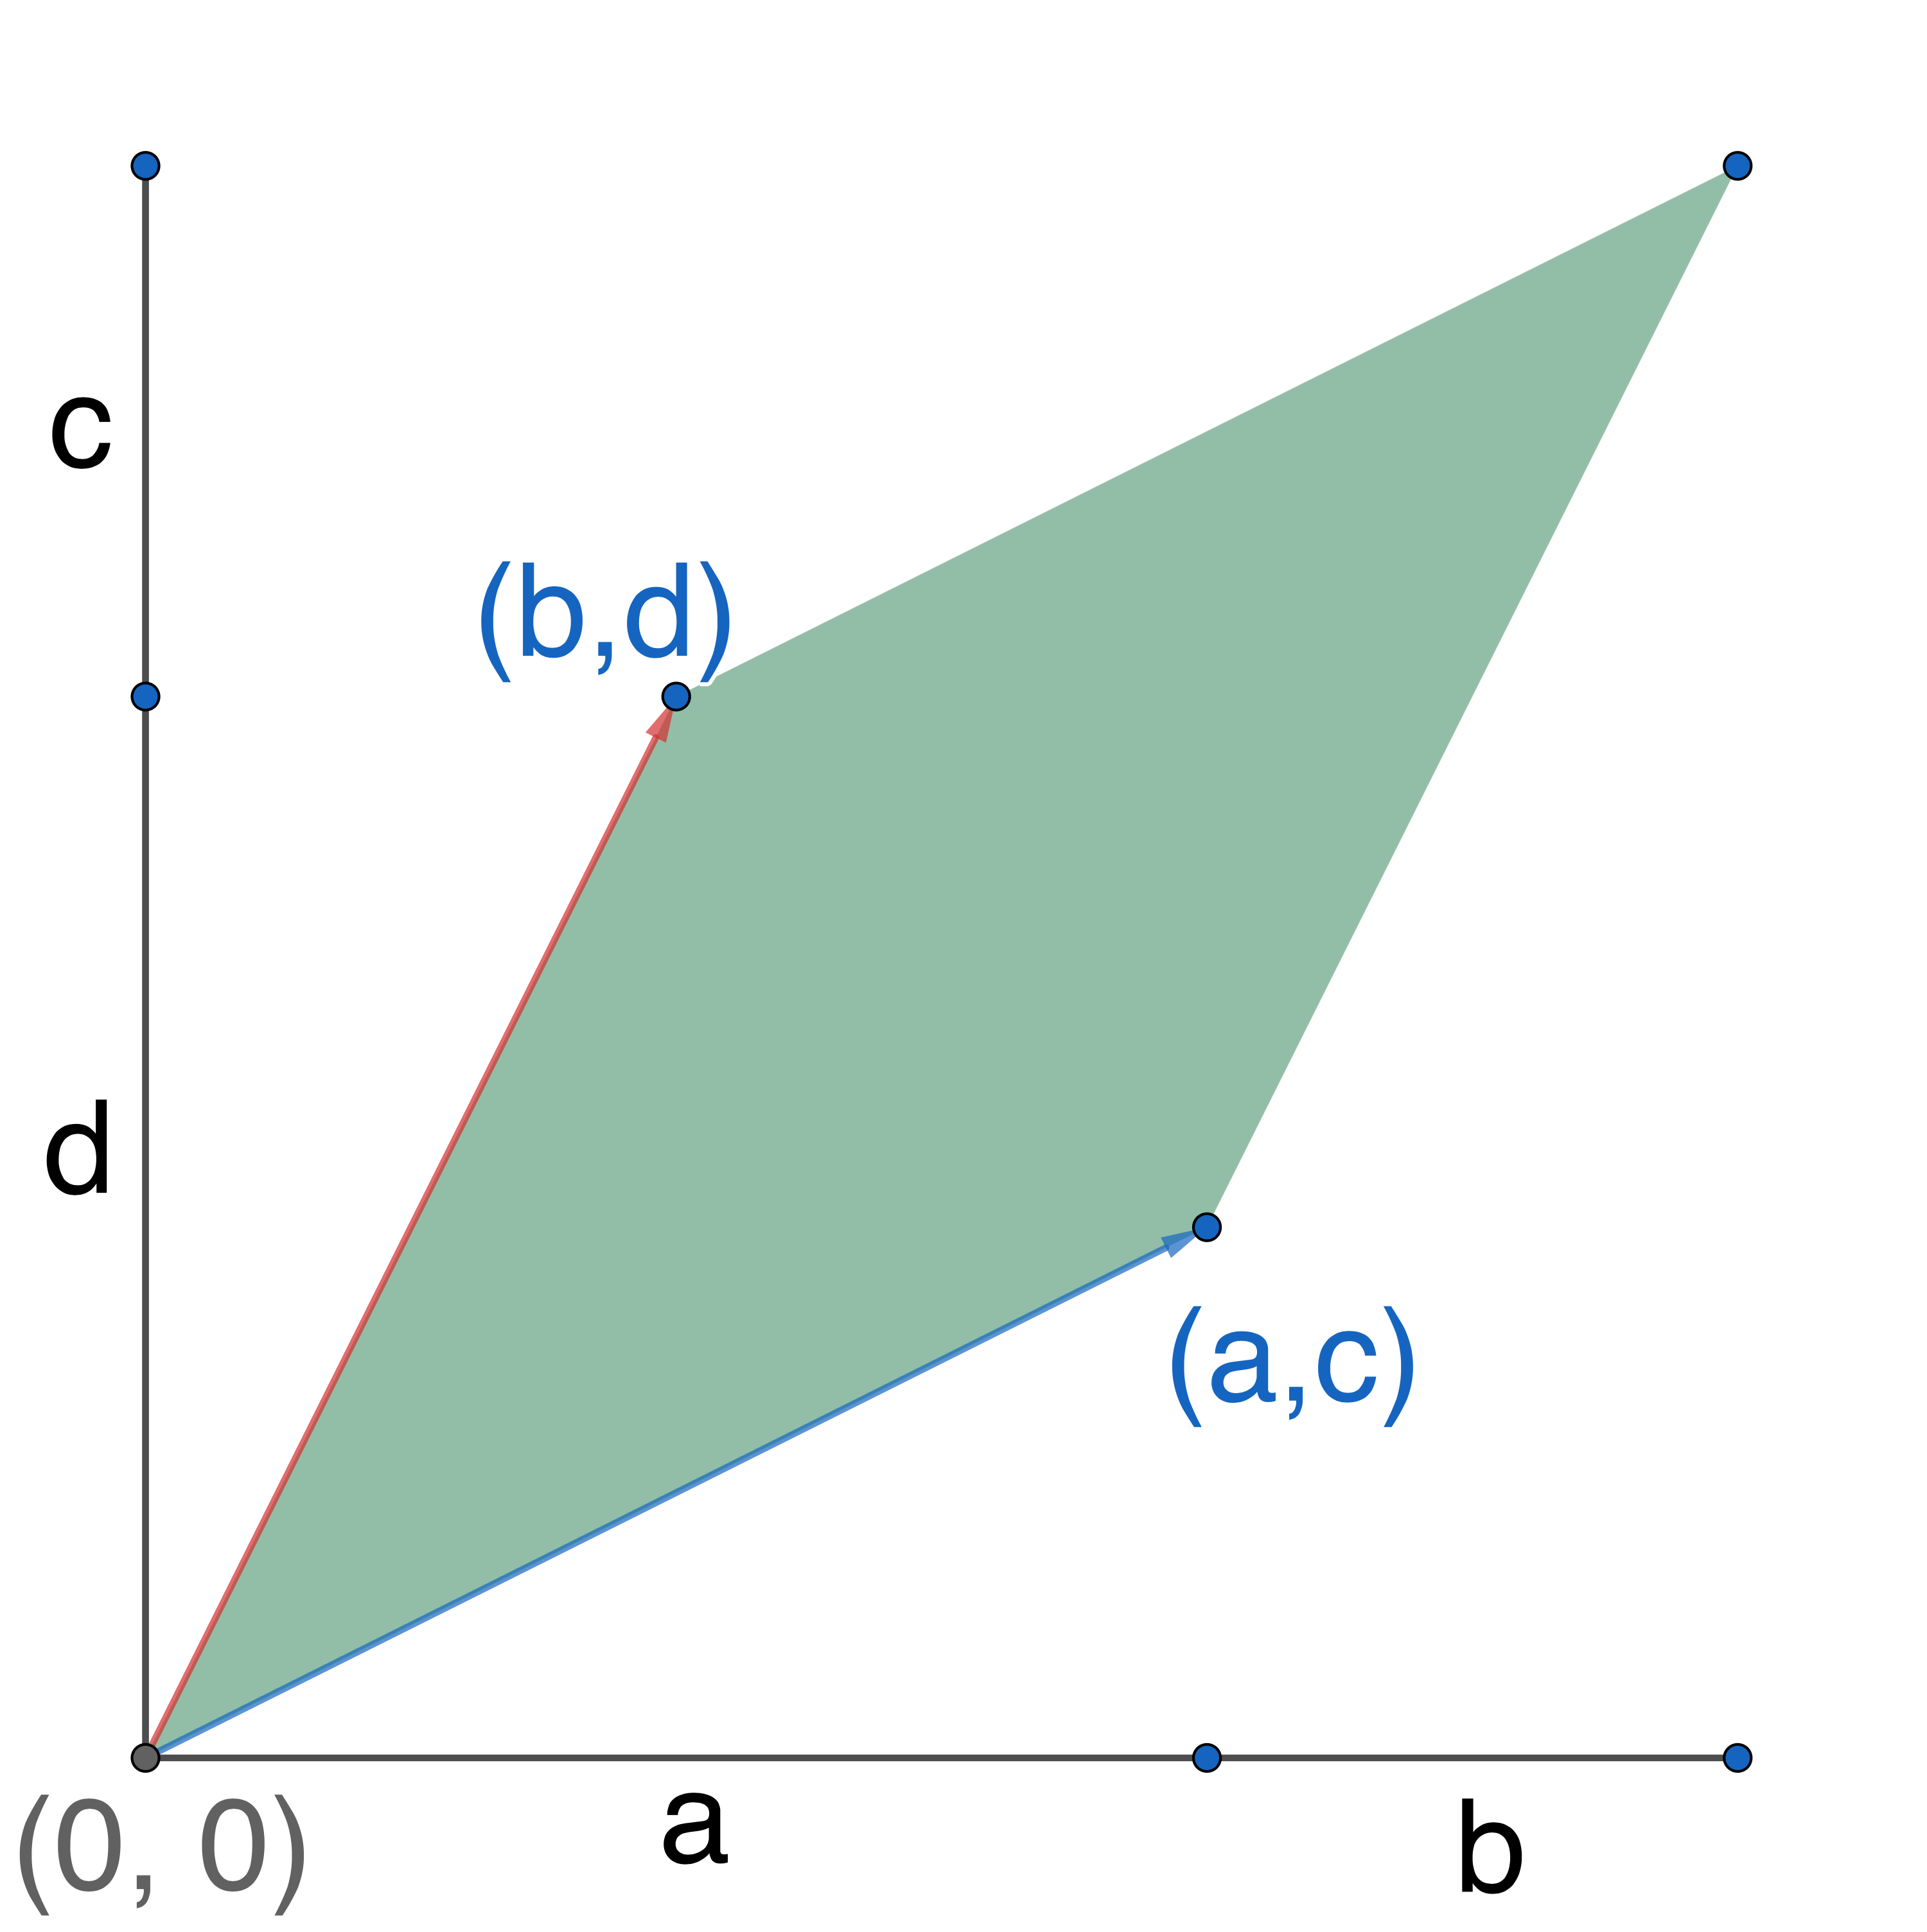
\includegraphics[height=0.8\textheight]{2018-09027geogebra-export.png}
      \column{.2\textwidth}
      \hspace{-2cm}
      \begin{align*}
        Area &= (a+b)(c+d)\\
             &-bc-bc\\
             &-\frac{1}{2}ac-\frac{1}{2}bd\\
             &-\frac{1}{2}ac-\frac{1}{2}bd\\
             &= ac+ad+bc+bd\\
             &-2bc-ac-bd\\
             &= ad-bc
      \end{align*}
    \end{columns}
  \end{figure}
\end{frame}

\begin{frame}{Examples}
  \begin{example}
    All identity matrices $I_n$ have determinant equal to $1$.
  \end{example}
  \begin{example}
    All matrices with repeated columns have determinant equal to $0$.
  \end{example}
  \begin{example}
    In fact a matrix is invertible iff its determinant is {\bf not} equal to $0$.
  \end{example}
\end{frame}


\begin{frame}{Effect of elementary row/column operations}
  The effect of the elementary row/column operations on $det(A)$ are:-\vfill
  \begin{itemize}
  \item Multiplying a row/column by a scalar $k$
    \begin{itemize}
    \item multiplies the determinant by $k$.
    \end{itemize}\vfill
  \item Swapping two rows/columns
    \begin{itemize}
    \item multiplies the determinant by $-1$.
    \end{itemize}\vfill
  \item Adding a multiple of one row/column to another
    \begin{itemize}
    \item has no effect on the determinant.
    \end{itemize}
  \end{itemize}\vfill
  Pictures on Jupyter notebook.
\end{frame}

\begin{frame}{Determinants of diagonal matrix and scalar multiple}
  \begin{example}[Diagonal matrices]
    \begin{equation*}
      det
      \left[
	\begin{array}{cccc}
          \lambda_1 &0&0&0\\
          0&\lambda_2&0&0\\
          0&0&\lambda_3&0\\
          0&0&0&\lambda_4
	\end{array}
      \right] = \lambda_1\lambda_2\lambda_3\lambda_4
    \end{equation*}
  \end{example}\vfill
  \begin{example}[Scalar multiple]
    If $A$ is an $n\times n$ matrix then
    \begin{equation*}
      det(kA) = k^n det(A)
    \end{equation*}
  \end{example}
\end{frame}

\begin{frame}{Determinant of triangular matrix}
  \begin{example}{Triangular matrix}
    \begin{align*}
      det
      \left[
	\begin{array}{cccc}
          \lambda_1 &a_{12}&a_{13}&a_{14}\\
          0&\lambda_2&a_{23}&a_{24}\\
          0&0&\lambda_3&a_{34}\\
          0&0&0&\lambda_4
	\end{array}
      \right] &=
      det
      \left[
	\begin{array}{cccc}
          \lambda_1 &0&0&0\\
          a_{21}&\lambda_2&0&0\\
          a_{31}&a_{32}&\lambda_3&0\\
          a_{41}&a_{42}&a_{43}&\lambda_4
	\end{array}
                                \right] \\
                    &=det
      \left[
	\begin{array}{cccc}
          \lambda_1 &0&0&0\\
          0&\lambda_2&0&0\\
          0&0&\lambda_3&0\\
          0&0&0&\lambda_4
	\end{array}
                 \right]\\
                    &=
      \lambda_1\lambda_2\lambda_3\lambda_4
    \end{align*}
  \end{example}
\end{frame}

\begin{frame}{Calculating the determinant using row/column operations}
  \begin{itemize}
  \item Start with a square matrix $A$.\vfill
  \item Perform row/column operations on $A$ to convert into triangular form.
    \begin{itemize}
    \item (Keep track of these because they can change the determinant!)
    \item If we ever get a zero row/column then the determinant is $0$.
    \end{itemize}\vfill
  \item Calculate the determinant of the resulting triangular matrix.
  \end{itemize}
\end{frame}

\begin{frame}
  Questions?
\end{frame}

\section{Examples}

\begin{frame}
  \begin{beamercolorbox}[sep=12pt,center]{part title}
    \usebeamerfont{section title}\insertsection\par
  \end{beamercolorbox}
\end{frame}

\begin{frame}{Examples}
  \begin{example}
    Find
    \begin{equation*}
      \left|
	\begin{array}{ccc}
          1&2&3\\
          0&5&6\\
          0&0&9
	\end{array}
      \right|
    \end{equation*}
  \end{example}
  \begin{example}
    Find
    \begin{equation*}
      \left|
        \begin{array}{ccc}
          -3&5&-6\\
          1&-1&3\\
          2&-4&1
        \end{array}
      \right|
    \end{equation*}
  \end{example}
\end{frame}

\begin{frame}{Examples}
  \begin{example}
    Find
    \begin{equation*}
      \left|
        \begin{array}{cccc}
          3&1&2&4\\
          -1&-3&8&0\\
          1&-1&5&5\\
          1&1&2&-1
        \end{array}
      \right|
    \end{equation*}
  \end{example}
  \begin{example}
    If
    \begin{equation*}
      \left|
        \begin{array}{ccc}
          a_1&a_2&a_3\\
          b_1&b_2&b_3\\
          c_1&c_2&c_3
        \end{array}
      \right| = 4 \text{ find }
      \left|
        \begin{array}{ccc}
          -b_1&-b_2&-b_3\\
          a_1+2b_1&a_2+2b_2&a_3+2b_3\\
          3c_1&3c_2&3c_3
        \end{array}
      \right|
    \end{equation*}
  \end{example}
\end{frame}

\begin{frame}{Examples}
  \begin{example}
    Find
    \begin{equation*}
      \left|
        \begin{array}{ccc}
          2&3&5\\
          3&5&9\\
          1&2&4
        \end{array}
      \right|
    \end{equation*}
  \end{example}
\end{frame}

\begin{frame}
  Questions?
\end{frame}

\section{Traditional determinants}

\begin{frame}
  \begin{beamercolorbox}[sep=12pt,center]{part title}
    \usebeamerfont{section title}\insertsection\par
  \end{beamercolorbox}
\end{frame}

\begin{frame}{Minors and cofactors}
  \begin{definition}
    Let $A = \left[a_{ij} \right]$ be an $n \times n$ matrix. 
    The \alert{$ij^{th}$ minor} of $A$, denoted as
    $minor\left( A\right) _{ij},$ is the determinant
    of the $n-1 \times n-1$ matrix which results from deleting the $i^{th}$ row and
    the $j^{th}$ column of $A$.
  \end{definition}

  \[
    A=
    \left[
      \begin{array}{rrrrrr}
        a_{11} & a_{12} & \cdots & \textcolor{red}{a_{1j}} & \cdots & a_{1n} \\
        a_{21} & a_{22} & \cdots & \textcolor{red}{a_{2j}} & \cdots & a_{2n} \\
        \vdots & \vdots & & \vdots & & \vdots \\
        \textcolor{blue}{a_{i1}} & \textcolor{blue}{a_{i2}} & \cdots & \textcolor{purple}{a_{ij}} & \cdots & \textcolor{blue}{a_{in}} \\
        \vdots & \vdots & & \vdots & & \vdots \\
        a_{n1} & a_{n2} & \cdots & \textcolor{red}{a_{nj}} & \cdots & a_{nn}
      \end{array}
    \right] 
  \]
\end{frame}

\begin{frame}{Examples}
  \begin{example}
    Find the (1,2)-minor of
    \begin{equation*}
      \left[
	\begin{array}{ccc}
          1&1&3\\
          2&4&1\\
          5&2&6
	\end{array}
      \right]
    \end{equation*}
  \end{example}
  \begin{example}
    Find the (2,2)-minor of
    \begin{equation*}
      \left[
	\begin{array}{cccc}
          1&5&2&5\\
          2&6&7&1\\
          9&9&8&2\\
          0&8&6&0
	\end{array}
      \right]
    \end{equation*}
  \end{example}
\end{frame}

\begin{frame}{Cofactors}
    \begin{definition}
    The \emph{$ij^{th}$ cofactor} of $A$ is
    \begin{equation*}
      \mbox{cof}(A)_{ij}=(-1)^{i+j} minor \left(A\right)_{ij}
    \end{equation*}
  \end{definition}
\end{frame}

\begin{frame}{Examples}
  \begin{example}
    Find the (1,2)-cofactor of
    \begin{equation*}
      \left[
	\begin{array}{ccc}
          1&1&3\\
          2&4&1\\
          5&2&6
	\end{array}
      \right]
    \end{equation*}
  \end{example}
  \begin{example}
    Find the (2,2)-cofactor of
    \begin{equation*}
      \left[
	\begin{array}{cccc}
          1&5&2&5\\
          2&6&7&1\\
          9&9&8&2\\
          0&8&6&0
	\end{array}
      \right]
    \end{equation*}
  \end{example}
\end{frame}

\begin{frame}{Recursive definition of determinant}
  \begin{definition}[Cofactor expansion along row i]
    \begin{align*}
      \det A &= \sum_{k=1}^n a_{ik}\mbox{cof}(A)_{ik}\\
             &=a_{i1} \mbox{cof}(A)_{i1} + a_{i2}\mbox{cof}(A)_{i2} +
      a_{i3}\mbox{cof}(A)_{i3} + \cdots + a_{in}\mbox{cof}(A)_{in}
    \end{align*}
  \end{definition}
  \begin{definition}[Cofactor expansion along column i]
    \begin{align*}
      \det A &= \sum_{k=1}^n a_{kj}\mbox{cof}(A)_{kj}\\
             &=a_{1j} \mbox{cof}(A)_{1j} + a_{2j}\mbox{cof}(A)_{2j} +
      a_{3j}\mbox{cof}(A)_{3j} + \cdots + a_{nj}\mbox{cof}(A)_{nj}
    \end{align*}
  \end{definition}
\end{frame}

\begin{frame}{Three dimensions}
  \begin{example}[Row 1 expansion]
    \begin{equation*}
      \left|
        \begin{array}{ccc}
          a_{11}&a_{12}&a_{13}\\
          a_{21}&a_{22}&a_{23}\\
          a_{31}&a_{32}&a_{33}
        \end{array}
      \right|=
      a_{11}\left|
	\begin{array}{cc}
          a_{22}&a_{23}\\
          a_{32}&a_{33}
	\end{array}
      \right|-a_{12} \left|
	\begin{array}{cc}
          a_{21}&a_{23}\\
          a_{31}&a_{33}
	\end{array}
      \right|+a_{13} \left|
	\begin{array}{cc}
          a_{21}&a_{22}\\
          a_{31}&a_{32}
	\end{array}
      \right|
    \end{equation*}
  \end{example}
   \begin{example}[Row 2 expansion]
    \begin{equation*}
      \left|
        \begin{array}{ccc}
          a_{11}&a_{12}&a_{13}\\
          a_{21}&a_{22}&a_{23}\\
          a_{31}&a_{32}&a_{33}
        \end{array}
      \right|=
      -a_{21}\left|
	\begin{array}{cc}
          a_{12}&a_{13}\\
          a_{32}&a_{33}
	\end{array}
      \right|+a_{22} \left|
	\begin{array}{cc}
          a_{11}&a_{13}\\
          a_{31}&a_{33}
	\end{array}
      \right|-a_{23} \left|
	\begin{array}{cc}
          a_{11}&a_{12}\\
          a_{31}&a_{32}
	\end{array}
      \right|
    \end{equation*}
  \end{example}
\end{frame}


\begin{frame}
  Questions?
\end{frame}

\section{Examples}

\begin{frame}
  \begin{beamercolorbox}[sep=12pt,center]{part title}
    \usebeamerfont{section title}\insertsection\par
  \end{beamercolorbox}
\end{frame}

\begin{frame}{Examples}
  
  \begin{example}
    Find
    \begin{equation*}
      \left|
	\begin{array}{ccc}
          1&1&3\\
          2&4&1\\
          5&2&6
	\end{array}
      \right|
    \end{equation*}
  \end{example}
\end{frame}

\begin{frame}{Examples}
  \begin{example}
    Find
    \begin{equation*}
      \left|
        \begin{array}{cccc}
          0&1&-2&1\\
          5&0&0&7\\
          0&1&-1&0\\
          3&0&0&2
        \end{array}
      \right|
    \end{equation*}
  \end{example}
  \begin{example}
    Find
    \begin{equation*}
      \left|
        \begin{array}{cccc}
          -8&1&0&-4\\
          5&7&0&-7\\
          12&-3&0&8\\
          -3&11&0&2
        \end{array}
      \right|
    \end{equation*}
  \end{example}
\end{frame}

\begin{frame}{Examples}
  \begin{example}
    Find
    \begin{equation*}
      det \left[
	\begin{array}{ccc}
          1&0&3\\
          1&0&1\\
          3&1&0               
	\end{array}
      \right]
    \end{equation*}
  \end{example}
    \begin{example}
    Find
    \begin{equation*}
      det \left[
	\begin{array}{ccc}
          1&2&3\\
          0&2&1\\
          2&6&7               
	\end{array}
      \right]
    \end{equation*}
  \end{example}
\end{frame}

\begin{frame}
  Questions?
\end{frame}

\end{document}